\documentclass[letterpaper]{article}
\usepackage[T1]{fontenc}
\usepackage[utf8]{inputenc}
\usepackage{tocloft,siunitx,amssymb,amsmath,graphicx,subcaption}
\usepackage[top=3cm,left=3cm,right=3cm,bottom=3cm]{geometry}
\usepackage{float,pgf,pgfplots}
\usepackage[american]{circuitikz}
\graphicspath{{img/}}
\renewcommand\cftsecfont{\normalfont}
\renewcommand\cftsecpagefont{\normalfont}
\renewcommand{\cftsecleader}{\cftdotfill{\cftsecdotsep}}
\renewcommand\cftsecdotsep{\cftdot}
\renewcommand\cftsubsecdotsep{\cftdot}
\renewcommand\cftsubsubsecdotsep{\cftdot}
\title{Lab 9: Thévenin's Theorem}
\author{
    Sebastián Nava López\\
    \and
    Ericka Sabrina Pensamiento R.\\
    \and
    Salvador Palos Gil
}
%\captionsetup[subfigure]{justification=raggedright}
\begin{document}
\begin{titlepage}
    \centering
    {\Huge Instituto Politécnico Nacional}\\[3ex]
    {\huge Escuela Superior de Cómputo}\\[8ex]
    {\huge Fundamental Circuit Analysis}\\[12ex]
    {\Large Lab 9: Thévenin's Theorem}\\[20ex]
    {\Large Group: 1CV5 Team: 7 \\[8ex]
    Sebastian Nava López\\[4ex]
    Sabrina Erika Pensamiento Robledo\\[4ex]
    Salvador Palos Gil\\[18ex]
    }
    \large{Elaboration: May 22, 2018\hspace{8em} Due date: May 29, 2018}
\end{titlepage}
\tableofcontents
\newpage
\section{Introduction}
\newpage
\section{Development}
\subsection{Calculations}
Using the circuit shown in Fig.\ref{fig:diag1}:
\begin{figure}[H]
    \centering
    \begin{circuitikz}[scale=0.75,transform shape]
        \draw (0,0) to [V = $\SI{5}{\volt}$,invert] (0,3)
        to [R = $\SI{1}{\kilo\ohm}$] (2,3)
        to [R = $\SI{470}{\ohm}$] (4,3)
        to [V = $\SI{20}{\volt}$,invert] (6,3)
        to [R = $\SI{1}{\kilo\ohm}$] (8,3)
        to [V = $\SI{10}{\volt}$,invert] (10,3)
        to [short,-*](11,3)
        (2,3) to [R = $\SI{1}{\kilo\ohm}$] (2,0)
        (8,3) to [R = $\SI{2.2}{\kilo\ohm}$] (8,0)
        (0,0) to [short,-*] (11,0);
        \draw {
            [anchor = south west](11,0) node {\textbf{B}}
            [anchor = south west](11,3) node {\textbf{A}}
        };
    \end{circuitikz}
    \caption{Circuit diagram}
    \label{fig:diag1}
\end{figure}
first we need to find Thévenin-equivalent resistance($R_{TH}$), in order to find it we need to
replace all the voltage sources with a short circuit, the resulting circuit is the one shown in
Fig.\ref{fig:diag2}:
\begin{figure}[H]
    \centering
    \begin{circuitikz}[scale=0.75,transform shape]
        \draw (0,0) -- (0,3)
        to [R = $\SI{1}{\kilo\ohm}$] (2,3)
        to [R = $\SI{470}{\ohm}$] (4,3)
        to [R = $\SI{1}{\kilo\ohm}$] (6,3)
        to [short,-*](9,3)
        (2,3) to [R = $\SI{1}{\kilo\ohm}$] (2,0)
        (6,3) to [R = $\SI{2.2}{\kilo\ohm}$] (6,0)
        (0,0) to [short,-*] (9,0);
        \draw {
            [anchor = south west](9,0) node {\textbf{B}}
            [anchor = south west](9,3) node {\textbf{A}}
        };
    \end{circuitikz}
    \caption{Resulting circuit after shorting the power sources}
    \label{fig:diag2}
\end{figure}
First we combine the \SI{1}{\kilo\ohm} and \SI{470}{\ohm} resistors located at the center of the
circuit, as they are connected in series, the equivalent resistor is equal to the sum of both
resistances.
\begin{figure}[H]
    \centering
    \begin{circuitikz}[scale=0.75,transform shape]
        \draw (0,0) -- (0,3)
        to [R = $\SI{1}{\kilo\ohm}$] (2,3)
        to [R = $\SI{1.47}{\kilo\ohm}$] (4,3)
        to [short,-*](7,3)
        (2,3) to [R = $\SI{1}{\kilo\ohm}$] (2,0)
        (4,3) to [R = $\SI{2.2}{\kilo\ohm}$] (4,0)
        (0,0) to [short,-*] (7,0);
        \draw {
            [anchor = south west](7,0) node {\textbf{B}}
            [anchor = south west](7,3) node {\textbf{A}}
        };
    \end{circuitikz}
\end{figure}
Then, we combine the \SI{1}{\kilo\ohm} and \SI{1}{\kilo\ohm} resistors that are wired in parallel,
the equivalent resistor is equal to
$\frac{\SI{1}{\kilo\ohm}\cdot\SI{1}{\kilo\ohm}}{2(\SI{1}{\kilo\ohm})} = \SI{500}{\ohm}$
\begin{figure}[H]
    \centering
    \begin{circuitikz}[scale=0.75,transform shape]
        \draw (0,0) -- (0,3)
        to [R = $\SI{500}{\ohm}$] (2,3)
        to [R = $\SI{1.47}{\kilo\ohm}$] (4,3)
        to [short,-*](7,3)
        (4,3) to [R = $\SI{2.2}{\kilo\ohm}$] (4,0)
        (0,0) to [short,-*] (7,0);
        \draw {
            [anchor = south west](7,0) node {\textbf{B}}
            [anchor = south west](7,3) node {\textbf{A}}
        };
    \end{circuitikz}
\end{figure}
Combining the \SI{500}{\ohm} and \SI{1.47}{\kilo\ohm} resistors, the equivalent resistor is equal
to $\SI{500}{\ohm}+\SI{1.47}{\kilo\ohm} = \SI{1.97}{\kilo\ohm}$
\begin{figure}[H]
    \centering
    \begin{circuitikz}[scale=0.75,transform shape]
        \draw (0,0) -- (0,3)
        to [R = $\SI{1.97}{\kilo\ohm}$] (2,3)
        to [short,-*](5,3)
        (2,3) to [R = $\SI{2.2}{\kilo\ohm}$] (2,0)
        (0,0) to [short,-*] (5,0);
        \draw {
            [anchor = south west](5,0) node {\textbf{B}}
            [anchor = south west](5,3) node {\textbf{A}}
        };
    \end{circuitikz}
\end{figure}
Finally, $R_{TH}$ is given by the equivalent resistance of the \SI{1.97}{\kilo\ohm} and
\SI{2.2}{\kilo\ohm} resistors connected in parallel:
\[\therefore R_{TH} =
\frac{\SI{1.97}{\kilo\ohm}\cdot\SI{2.2}{\kilo\ohm}}{\SI{1.97}{\kilo\ohm}+\SI{2.2}{\kilo\ohm}}\ =
\SI{1039.328}{\ohm}\]
To find the Thévenin-equivalent voltage we need to find the voltage passing in nodes $A$ and $B$,
we choose to simplify the circuit using the source transformation method.
First we transform the \SI{5}{\volt} source to a current source:
\[I_S = \frac{\SI{5}{\volt}}{\SI{1}{\kilo\ohm}}\ = \SI{5}{\milli\ampere}\]
\begin{figure}[H]
    \centering
    \begin{circuitikz}[scale=0.75,transform shape]
        \draw (0,0) to [I,label = $\SI{5}{\milli\ampere}$] (0,3) -- (4,3)
        (4,3) to [R = $\SI{470}{\ohm}$] (6,3)
        to [V = $\SI{20}{\volt}$,invert] (8,3)
        to [R = $\SI{1}{\kilo\ohm}$] (10,3)
        to [V = $\SI{10}{\volt}$,invert] (12,3)
        to [short,-*](13,3)
        (2,3) to [R = $\SI{1}{\kilo\ohm}$] (2,0)
        (4,3) to [R = $\SI{1}{\kilo\ohm}$] (4,0)
        (10,3) to [R = $\SI{2.2}{\kilo\ohm}$] (10,0)
        (0,0) to [short,-*] (13,0);
        \draw {
            [anchor = south west](13,0) node {\textbf{B}}
            [anchor = south west](13,3) node {\textbf{A}}
        };
    \end{circuitikz}
\end{figure}
Merging the \SI{1}{\kilo\ohm} resistor and the \SI{1}{\kilo\ohm} resistor connected in parallel yields a
equivalent resistor equal to:
\[R_{eq} = \frac{(\SI{1}{\kilo\ohm})(\SI{1}{\kilo\ohm})}{2(\SI{1}{\kilo\ohm})} = \SI{500}{\ohm}\]
\begin{figure}[H]
    \centering
    \begin{circuitikz}[scale=0.75,transform shape]
        \draw (0,0) to [I,label = $\SI{5}{\milli\ampere}$] (0,3) -- (2,3)
        (2,3) to [R = $\SI{470}{\ohm}$] (4,3)
        to [V = $\SI{20}{\volt}$,invert] (6,3)
        to [R = $\SI{1}{\kilo\ohm}$] (8,3)
        to [V = $\SI{10}{\volt}$,invert] (10,3)
        to [short,-*](11,3)
        (2,3) to [R = $\SI{500}{\ohm}$] (2,0)
        (8,3) to [R = $\SI{2.2}{\kilo\ohm}$] (8,0)
        (0,0) to [short,-*] (11,0);
        \draw {
            [anchor = south west](11,0) node {\textbf{B}}
            [anchor = south west](11,3) node {\textbf{A}}
        };
    \end{circuitikz}
\end{figure}
Next we transform the \SI{5}{\milli\ampere} current source to a voltage source:
\[V_S = \SI{5}{\milli\ampere}\cdot\SI{500}{\ohm} = \SI{2.5}{\volt}\]
\begin{figure}[H]
    \centering
    \begin{circuitikz}[scale=0.75,transform shape]
        \draw (0,0) to [V,label = $\SI{2.5}{\volt}$,invert] (0,3)
        to [R = $\SI{500}{\ohm}$] (2,3)
        to [R = $\SI{470}{\ohm}$] (4,3)
        to [V = $\SI{20}{\volt}$,invert] (6,3)
        to [R = $\SI{1}{\kilo\ohm}$] (8,3)
        to [V = $\SI{10}{\volt}$,invert] (10,3)
        to [short,-*](11,3)
        (8,3) to [R = $\SI{2.2}{\kilo\ohm}$] (8,0)
        (0,0) to [short,-*] (11,0);
        \draw {
            [anchor = south west](11,0) node {\textbf{B}}
            [anchor = south west](11,3) node {\textbf{A}}
        };
    \end{circuitikz}
\end{figure}
Combining the \SI{500}{\ohm} and \SI{470}{\ohm} resistors connected in series:
\[R_{EQ} = \SI{500}{\ohm}+\SI{470}{\ohm} = \SI{970}{\ohm}\]
\begin{figure}[H]
    \centering
    \begin{circuitikz}[scale=0.75,transform shape]
        \draw (0,0) to [V,label = $\SI{2.5}{\volt}$,invert] (0,3)
        to [R = $\SI{970}{\ohm}$] (2,3)
        to [V = $\SI{20}{\volt}$,invert] (4,3)
        to [R = $\SI{1}{\kilo\ohm}$] (6,3)
        to [V = $\SI{10}{\volt}$,invert] (8,3)
        to [short,-*](9,3)
        (6,3) to [R = $\SI{2.2}{\kilo\ohm}$] (6,0)
        (0,0) to [short,-*] (9,0);
        \draw {
            [anchor = south west](9,0) node {\textbf{B}}
            [anchor = south west](9,3) node {\textbf{A}}
        };
    \end{circuitikz}
\end{figure}
Changing the order of the components and combining resistors and voltage sources we have:
\begin{gather*}
    V_S = \SI{22.5}{\volt}\\
    R_{EQ} = \SI{1}{\kilo\ohm}+\SI{970}{\ohm} = \SI{1.97}{\kilo\ohm}
\end{gather*}
\begin{figure}[H]
    \centering
    \begin{circuitikz}[scale=0.75,transform shape]
        \draw (0,0) to [V,label = $\SI{22.5}{\volt}$,invert] (0,3)
        to [R = $\SI{1.97}{\kilo\ohm}$] (3,3)
        to [V = $\SI{10}{\volt}$,invert] (6,3)
        to [short,-*](6,3)
        (3,3) to [R = $\SI{2.2}{\kilo\ohm}$] (3,0)
        (0,0) to [short,-*] (6,0);
        \draw {
            [anchor = south west](6,0) node {\textbf{B}}
            [anchor = south west](6,3) node {\textbf{A}}
        };
    \end{circuitikz}
\end{figure}
Transforming the voltage source into a current source:
\[I_S = \frac{\SI{22.5}{\volt}}{\SI{1.97}{\kilo\ohm}} = \SI{11.421}{\milli\ampere}\]
\begin{figure}[H]
    \centering
    \begin{circuitikz}[scale=0.75,transform shape]
        \draw (0,0) to [I,label = $\SI{11.421}{\milli\ampere}$] (0,3) -- (4,3)
        (4,3) to [V = $\SI{10}{\volt}$,invert] (7,3)
        to [short,-*](7,3)
        (2,3) to [R = $\SI{1.97}{\kilo\ohm}$] (2,0)
        (4,3) to [R = $\SI{2.2}{\kilo\ohm}$] (4,0)
        (0,0) to [short,-*] (7,0);
        \draw {
            [anchor = south west](7,0) node {\textbf{B}}
            [anchor = south west](7,3) node {\textbf{A}}
        };
    \end{circuitikz}
\end{figure}
Combining the parallel resistors we have that:
\[R_{EQ} =
\frac{\SI{1.97}{\kilo\ohm}\cdot\SI{2.2}{\kilo\ohm}}{\SI{1.97}{\kilo\ohm}+\SI{2.2}{\kilo\ohm}} =
\SI{1039.328}{\ohm}\]
\begin{figure}[H]
    \centering
    \begin{circuitikz}[scale=0.75,transform shape]
        \draw (0,0) to [I,label = $\SI{11.421}{\milli\ampere}$] (0,3) -- (2,3)
        (2,3) to [V = $\SI{10}{\volt}$,invert] (5,3)
        to [short,-*](5,3)
        (2,3) to [R = $\SI{1039}{\ohm}$] (2,0)
        (0,0) to [short,-*] (5,0);
        \draw {
            [anchor = south west](5,0) node {\textbf{B}}
            [anchor = south west](5,3) node {\textbf{A}}
        };
    \end{circuitikz}
\end{figure}
Transforming the current source to a voltage source:
\[V_S = (\SI{11.421}{\milli\ampere})(\SI{1039.328}{\ohm}) = \SI{11.870}{\volt}\]
\begin{figure}[H]
    \centering
    \begin{circuitikz}[scale=0.75,transform shape]
        \draw (0,0) to [V,label = $\SI{11.87}{\volt}$,invert] (0,3)
        to [R = $\SI{1039}{\ohm}$](2,3)
        to [V = $\SI{10}{\volt}$,invert] (5,3)
        to [short,-*](5,3)
        (0,0) to [short,-*] (5,0);
        \draw {
            [anchor = south west](5,0) node {\textbf{B}}
            [anchor = south west](5,3) node {\textbf{A}}
        };
    \end{circuitikz}
\end{figure}
Then we change the order of series elements and merging both voltage sources:
\[V_S = \SI{11.870}{\volt}+\SI{10}{\volt} = \SI{21.870}{\volt}\]
\begin{figure}[H]
    \centering
    \begin{circuitikz}[scale=0.75,transform shape]
        \draw (0,0) to [V,label = $\SI{21.87}{\volt}$,invert] (0,3)
        to [R = $\SI{1039}{\ohm}$,-*](4,3)
        (0,0) to [short,-*] (4,0);
        \draw {
            [anchor = south west](4,0) node {\textbf{B}}
            [anchor = south west](4,3) node {\textbf{A}}
        };
    \end{circuitikz}
\end{figure}
Finally, the Thévenin-equivalent voltage is equal to:
\[\therefore V_{TH} = \SI{21.87}{\volt}\]
The current going along nodes $A$ and $B$ is given by:
\[I_{AB} = \frac{V_{TH}}{R_{TH}} = \frac{\SI{21.870}{\volt}}{\SI{1039.328}{\ohm}} =
\SI{21.649}{\milli\ampere}\]
When the load resistor($R_L$) is connected, the voltage in the resistor is given by:
\[V_L = R_L\Bigg(\frac{V_{TH}}{R_{TH}+R_L}\Bigg) =
\SI{3.3}{\kilo\ohm}\Bigg(\frac{\SI{21.870}{\volt}}{\SI{1039.328}{\ohm}+\SI{3.3}{\kilo\ohm}}\Bigg)
= \SI{16.632}{\volt}\]
The current in the resistor is:
\[I_L = \frac{V_L}{R_L} = \frac{\SI{16.632}{\volt}}{\SI{3.3}{\kilo\ohm}} =
\SI{5.040}{\milli\ampere}\]
Power in the resistor is given by:
\[P_L = I_L\cdot\ V_L = (\SI{5.040}{\milli\ampere})(\SI{16.632}{\volt}) = \SI{0.083}{\watt}\]
\subsection{Simulation}
\begin{figure}[H]
    \centering
    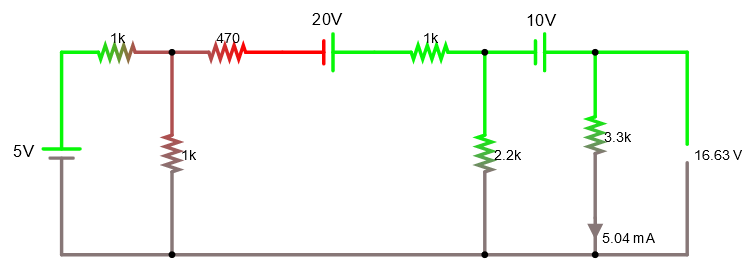
\includegraphics[width=.85\linewidth]{sim1}
    \caption{Circuit with load resistor($R_L$)}
\end{figure}
\begin{figure}[H]
    \centering
    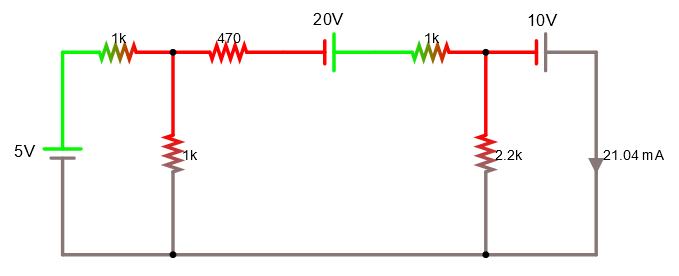
\includegraphics[width=.85\linewidth]{sim2}
    \caption{Circuit without load resistor($R_L$), current measurement}
\end{figure}
\begin{figure}[H]
    \centering
    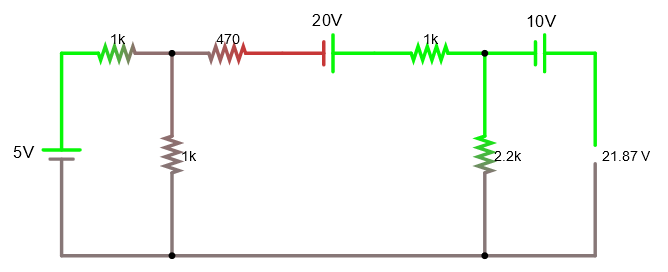
\includegraphics[width=.85\linewidth]{sim3}
    \caption{Circuit without load resistor($R_L$), voltage measurement}
\end{figure}
\begin{figure}[H]
    \centering
    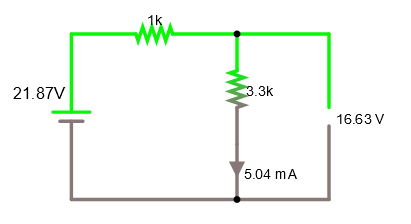
\includegraphics[width=.5\linewidth]{sim4}
    \caption{Circuit with Thévenin-equivalent voltage and resistor}
\end{figure}
\subsection{Measurements}
\begin{figure}[H]
    \centering
    \begin{circuitikz}[scale=0.75,transform shape]
        \draw (0,0) to [V = $\SI{5}{\volt}$,invert] (0,3)
        to [R = $\SI{1}{\kilo\ohm}$] (2,3)
        to [R = $\SI{470}{\ohm}$] (4,3)
        to [V = $\SI{20}{\volt}$,invert] (6,3)
        to [R = $\SI{1}{\kilo\ohm}$] (8,3)
        to [V = $\SI{10}{\volt}$,invert] (10,3)
        to [short,-*](11,3)
        (2,3) to [R = $\SI{1}{\kilo\ohm}$] (2,0)
        (8,3) to [R = $\SI{2.2}{\kilo\ohm}$] (8,0)
        (11,3) to [R = $R_L:\SI{3.3}{\kilo\ohm}$] (11,0)
        (0,0) to [short,-*] (11,0);
        \draw {
            [anchor = south west](11,0) node {\textbf{B}}
            [anchor = south west](11,3) node {\textbf{A}}
        };
    \end{circuitikz}
    \caption{Diagram of the first circuit}
    \label{fig:diag3}
\end{figure}
First, using the circuit shown in Fig.\ref{fig:diag3} , we measured current and voltage values in
the load resistor $R_L$:
\begin{table}[H]
    \centering
    \begin{tabular}{|c|c|c|c|}
        \hline
        Measurements & Theoretical value & Measured value & Simulated value \\\hline
        $I_L$ & \SI{5.040}{\milli\ampere} & \SI{5.000}{\milli\ampere} & \SI{5.040}{\milli\ampere}\\\hline
        $V_L$ & \SI{16.632}{\volt} & \SI{16.780}{\volt} & \SI{16.632}{\volt}\\\hline
        $P_L$ & \SI{0.083}{\watt} & \SI{0.083}{\watt} & \SI{}{\watt}\\\hline
    \end{tabular}
    \caption{Current, power and voltage values in load resistor($R_L$)}
\end{table}
Then we retired the load resistor and measured voltage and current between nodes $A$ and $B$:
\begin{table}[H]
    \centering
    \begin{tabular}{|c|c|c|c|}
        \hline
        Measurements & Theoretical value & Measured value & Simulated value \\\hline
        $I_{AB}$ & \SI{21.649}{\milli\ampere} & \SI{21.200}{\milli\ampere} & \SI{5.040}{\milli\ampere}\\\hline
        $V_{AB}$ & \SI{21.870}{\volt} & \SI{21.800}{\volt} & \SI{16.632}{\volt}\\\hline
        $R_{TH} = \frac{V_{AB}}{I_{AB}}$ & \SI{1039.328}{\ohm} & \SI{1028.300}{\ohm} & \SI{}{\ohm}\\\hline
    \end{tabular}
    \caption{Current, resistance and voltage values between nodes $A$ and $B$}
\end{table}
Finally we assembled a circuit as shown in Fig.\ref{fig:diag4}:
\begin{figure}[H]
    \centering
    \begin{circuitikz}
        \draw (0,0) to [V = $V_{TH}:\SI{21.87}{\volt}$,invert](0,2)
        to [R = $R_{TH}:\SI{1039.328}{\ohm}$] (2,2)
        to [R = $R_L:\SI{3.3}{\kilo\ohm}$] (2,0) -- (0,0);
    \end{circuitikz}
    \caption{Circuit using Thévenin-equivalent components}
    \label{fig:diag4}
\end{figure}
To reproduce the effect of the Thévenin-equivalent resistor($R_{TH}$) we used a potentiometer
adjusted to the value of $R_{TH}$, in this case, we measured current and voltage values flowing
through the load resistor($R_L$):
\begin{table}[H]
    \centering
    \begin{tabular}{|c|c|c|c|}
        \hline
        Measurements & Theoretical value & Measured value & Simulated value \\\hline
        $I_L$ & \SI{5.040}{\milli\ampere} & \SI{5.000}{\milli\ampere} & \SI{5.040}{\milli\ampere}\\\hline
        $V_L$ & \SI{16.632}{\volt} & \SI{16.780}{\volt} & \SI{16.670}{\volt}\\\hline
        $P_L$ & \SI{0.083}{\watt} & \SI{0.083}{\watt} & \SI{}{\watt}\\\hline
    \end{tabular}
    \caption{Current, power and voltage values in load resistor($R_L$) using Thévenin-equivalent
    components}
\end{table}
\section{Questions}
\textit{\textbf{Explain the operation of the oscilloscope}}\\
%ans
\textit{\textbf{What's the function of the signal generator?}}\\
%ans
\textit{\textbf{What are the Lissajous graphs for?}}\\
%ans
\textit{\textbf{What are the operating modes Y (t) and XY used for?}}\\
%ans
\textit{\textbf{Which means by coupling in D.C.?}}\\
%ans
\textit{\textbf{What is an offset signal?}}\\
%ans
\textit{\textbf{Which means that a signal is out of phase?}}\\
%ans
\section{Conclusions}
{\large\textbf{Sabrina:}}\\
%
\\[2ex]
{\large\textbf{Salvador:}}\\
%
\\[2ex]
{\large\textbf{Sebastián:}}\\
In this experiment we measured the current and voltage output in a pair of terminals in our
circuit, as well as in the terminal connected to this terminals, known as load resistor, then we found the Thévenin-equivalent($R_{TH}$) resistor doing the respective process, and the
Thévenin-equivalent voltage($V_{TH}$) using source transformation to find the voltage going through the
established terminals, with this information we found that assembling a circuit using a voltage
source with the voltage value of $V_{TH}$ and a resistor connected in series with the resistance
value of $R_{TH}$ had the same voltage and current when the ends of the resistor and the voltage
source are connected to a voltmeter or a ammeter, therefore when the load resistor was connected
to the terminals the current and voltage values through the resistor were the same as when the
resistor was connected to the complete circuit, thus verifying Thévenin's theorem.
\end{document}
